\newcommand{\CLASSINPUTbaselinestretch}{1.0} % baselinestretch
\newcommand{\CLASSINPUTinnersidemargin}{0.75in} % inner side margin
\newcommand{\CLASSINPUToutersidemargin}{0.75in} % outer side margin
\newcommand{\CLASSINPUTtoptextmargin}{0.75in}   % top text margin
\newcommand{\CLASSINPUTbottomtextmargin}{0.75in}% bottom text margin

\newcommand{\revised}[1]{{\color{blue}#1}}

\documentclass[conference]{IEEEtran}

\IEEEoverridecommandlockouts % precisa para usar o \thanks{}
% *** CITATION PACKAGES ***
%
\usepackage{cite}
\usepackage{flushend}
\usepackage{xcolor}
\usepackage[pdftex]{graphicx}

\usepackage[utf8]{inputenc}


% *** MATH PACKAGES ***
%
%\usepackage[cmex10]{amsmath}
\usepackage{amsmath}
\usepackage{amssymb}

% *** SPECIALIZED LIST PACKAGES ***
%
\usepackage{algorithm}
\usepackage{algorithmic}

% *** ALIGNMENT PACKAGES ***
%
\usepackage{array}
\usepackage{multirow}

% *** SUBFIGURE PACKAGES ***
\usepackage[tight,footnotesize]{subfigure}

% *** PDF, URL AND HYPERLINK PACKAGES ***
%
%\usepackage[bookmarks=false]{hyperref}
\usepackage{url}

% correct bad hyphenation here
\hyphenation{rep-re-sen-ta-tion fe-de-ral}


\begin{document}
%
% paper title
% can use linebreaks \\ within to get better formatting as desired
\title{\vspace{0.25in}Avaliação estatística sobre seleção de características para categorização de texto}


% author names and affiliations
% use a multiple column layout for up to three different
% affiliations

\author{\IEEEauthorblockN{
		Rog\'{e}rio C. P. Fragoso\IEEEauthorrefmark{1}, 
		Lucas F. Melo\IEEEauthorrefmark{1},
		Saulo C. R. P. Sobrinho\IEEEauthorrefmark{1}
}
\IEEEauthorblockA{Universidade Federal de Pernambuco (UFPE), Centro de Inform\'{a}tica (CIn)\\
Av. Jornalista Anibal Fernandes s/n, Cidade Universit\'{a}ria 50740-560, Recife, PE, Brazil\\
rcpf@cin.ufpe.br, lfm2@cin.ufpe.br, scrps@cin.ufpe.br \\}}
%\IEEEauthorrefmark{1}Telephone: +55 81 2126-8430 Ext.4346 Fax: +55 81 2126-8438}}

% make the title area
\maketitle

\begin{abstract}
	%\boldmath
\textcolor{red}{ESCREVER RESUMO}
\end{abstract}

\IEEEpeerreviewmaketitle

% Formato descrito na página da disciplina. Lá ela diz que a presença destas seções é mandatória. 
% (Acho que a gente não precisa organizar nesse formato exatamente, mas precisamos garantir que cada item esteja presente)

%•       Passo 1 – Justificativa: De início, explicitam-se os motivos que justificam a pesquisa, determinando-se e delimitando-se o problema, o qual deve estar formulado de maneira clara e precisa.
%•       Passo 2 - Fundamentação teórica: Descreve-se  o relacionamento do problema com a teoria que será utilizada na pesquisa.
%•       Passo 3 - Objetivo da pesquisa: Os objetivos devem ser retirados diretamente dos problemas levantados no Passo 2. Define-se o que se pretende alcançar com a realização do trabalho.
%•       Passo 4 - Especificação da amostra: Deve-se determinar a área de execução da pesquisa, a população a ser investigada, o tipo de amostra e a determinação do seu tamanho, bem como o tipo de amostragem a ser utilizado. Define-se as variáveis envolvidas.
%•       Passo 5– Análise exploratória: Fazer um estudo descritivo dos dados (gráficos e medidas).  Verificar normalidade dos dados e potenciais pontos aberrantes.
%•       Passo 6– Metodologia (Formulação das hipóteses): Estabelecem-se as hipóteses que serão formuladas, as quais devem ser claras e precisas. Define-se o problema estatisticamente, decidindo-se que informação estatística é realmente necessária e qual método que será aplicado.   
%•       Passo 7 - Análise dos resultados: Passa-se ao tratamento dos dados por intermédio dos testes estatísticos, os quais dependem das hipóteses que serão testadas. Nesse tópico, é exigido que sejam aplicados testes de hipóteses paramétricos e/ou não paramétricos. Testes de duas amostras são exigidos, quando comparando abordagens.

\section{Introdução}
\label{sec:intro}

Algoritmos são sequências de instruções bem definidas, porém suas implementações podem apresentar comportamentos difíceis de serem previstos.
Seja pelo uso de geração de números pseudo-aleatórios que geram um comportamento não determinístico inerente ao código, ou pelo uso de linguagens de alto nível cuja tradução para linguagem de máquina passa por otimizações e diferentes interações com a arquitetura de destino na qual o algoritmo é executado.
Sendo assim, a performance de algoritmos de computação em geral é não-determinística e, ao analisar comparativamente o desempenho destes algoritmos, é necessário levar em consideração que estamos diante de uma amostra aleatória que representa estas performances.

Este trabalho realiza uma comparação entre algoritmos de categorização de texto, mostrando como determinar e aplicar testes estatísticos adequados para este cenário.

\subsection{Fundamentação teórica}
%Seguindo o modelo sugerido no site, essa seção é obrigatória.

Na abordagem de aprendizagem de máquina, uma instância é representada como um vetor composto por pares de característica e valor. Uma abordagem comum para a representação de textos na forma de vetores de características é a técnica conhecida como \emph{Bag of Words} (BoW)~\cite{guyon2003introduction}. Nela, um texto é tratado como um conjunto de palavras, sem considerar gramática ou ordem de ocorrência das palavras no texto. Cada palavra do vocabulário da base de dados é considerada uma característica e é associada à frequência desta palavra no documento. Ou seja, o tamanho do vocabulário da base de dados define a dimensionalidade dos vetores. Desta forma, em uma base de dados de tamanho médio, é comum que os vetores de características contenham dezenas de milhares de dimensões~\cite{gabrilovich2004text}. Entretanto, a maior parte deestas características é irrelevante ou redundante. A alta dimensionalidade pode tornar a categorização de textos muito dispendiosa em termos de memória e tempo de execução. Adicionalmente, este grande número de características pode impactar negativamente no desempenho de classificação, especialmente em bases de dados com um número pequeno de instâncias em relação ao número de características, fenômeno conhecido como ``praga da dimensionalidade''. Como muitas das características são irrelevantes para a categorização, estes problemas podem ser tratados através da restrição da quantidade de características do conjunto de dados. Esta abordagem é conhecida como Redução de Dimensionalidade (DR, do inglês \emph{Dimensionality Reduction}).

Uma técnica de DR muito utilizada é a seleção de características. Nesta abordagem, o conjunto final é formado por parte das características do conjunto original. A utilização de métodos de filtragem é a técnica de FS considerada mais adequada para problemas de TC, devido ao custo computacional ser bem mais baixo que o de outras técnicas, como métodos \emph{wrapper}. Métodos de filtragem realizam um ordenamento das características através do uso de algoritmos determinísticos e métricas estatísticas, conhecidas com funções de avaliação de características (FEF, do inglês \emph{Feature Evaluation Function}). Após o ordenamento, uma quantidade, estabelecida pelo usuário, de características é selecionada para a formação do novo subconjunto.

\subsection{Métodos de seleção de características}
\label{sec:metodos}

\textit{Maximum f features per Document} (MFD)~\cite{mfd2014}, \textit{Maximum f features per Document-Reduced} (MFDR)~\cite{mfd2014} e \textit{Class-dependent Maximum f features per Document-Reduced} (cMFDR)~\cite{fragoso2016cmfdr} são métodos de seleção de características para categorização de texto. Estes métodos necessitam requerem um valor para o parâmetro $f$, que indica a quantidade de características a serem selecionadas por instância. A escolha de um bom valor para este parâmetro pode ser um trabalho demorado e exaustivo. Neste contexto, o método \textit{Automatic Feature Subsets Analyzer} (ASFA)~\cite{fragoso2016afsa} foi proposto como para ser usado conjuntamente com um dos três métodos: MFD, MFDR ou cMFDR. O objetivo do AFSA é prover, para estes métodos, um valor para o parâmetro $f$ de forma automática.

Esta seção apresentou conceitos básicos de categorização de textos e seleção de características e introduziu os quatro métodos de seleção de características que são avaliados no trabalho. 
O restante do trabalho é organizado como segue: 
A Seção \ref{sec:objetivo} apresenta o objetivo do presente trabalho. 
Na Seção \ref{sec:exp} são detalhadas as configurações dos experimentos, incluindo descrição da base de dados, os algoritmos de interesse e as hipóteses a serem verificadas sobre os dados. 
A Seção \ref{sec:analise} demonstra os procedimentos estatísticos realizados no trabalho.
Finalmente, a Seção \ref{sec:conclusao} apresenta as conclusões do trabalho.

\section{Objetivo}
\label{sec:objetivo}

O objetivo da presente pesquisa é verificar se o método AFSA é capaz de prover uma configuração para MFD, MFDR e cMFDR de modo que o desempenho de classificação não seja prejudicado. Ou seja, desejamos averiguar se o desempenho dos métodos MFD, MFDR e cMFDR é alterado quando estes métodos são usados conjuntamente com AFSA.
Esta análise comparativa visa determinar se os algoritmos possuem desempenhos significativamente diferentes e, em caso positivo, determinar qual apresenta desempenho superior.

%Para tanto, executamos análises estatísticas para avaliar a aderência dos dados amostrais a uma distribuição normal.
%Posteriormente, aplicamos testes de hipóteses adequados para, efetivamente, comparar os desempenho dos métodos.

\section{Experimentos}
\label{sec:exp}

Esta seção descreve as configurações dos experimentos realizados para gerar o conjunto de dados sobre o qual a análise será realizada.

\subsection{Base de dados}
\label{sec:bd}

Para a categorização de texto, foi utilizada a base de dados \textit{Reuters 10}.
Esta base de dados é um subconjunto da coleção \textit{Reuters-21578}~\footnote{Disponível em http://disi.unitn.it/moschitti/corpora.htm.}, que é uma das bases mais utilizadas em trabalhos de categorização de texto.
A base é composta por documentos coletados do \textit{Reuters newswire} de 1987 e apresenta 135 categorias.
Entretanto, o subconjunto adotado neste trabalho é composto pelas 10 maiores categorias da base.
O base de dados \textit{Reuters 10} contém 9.980 documentos e seu vocabulário abarca 10.987 termos.
A base de dados \textit{Reuters 10} também é muito utilizada em trabalhos de categorização de texto~\cite{chang2008multilabel,chen2009feature,yang2011new}. 

A distribuição dos documentos é bastante desbalanceada, apresentando categorias representando desde 2,3\% até 39\% do tamanho total da base. 
Nesta base foram aplicados os seguintes procedimentos de pré-processamento: \textit{stemming}, com o algoritmo \textit{Iterated Lovins Stemmer}~\cite{lovins1968development}, 
remoção de termos com duas ou menos letras e remoção de \textit{stopwords}.

Vale salientar que  a análise comparativa deste trabalho é realizada sobre o desempenho dos algoritmos, tendo a base citada como entrada, e não sobre características da base em si. O processo de geração das amostras utilizadas na análise estatística é detalhado na Seção~\ref{sec:metodologia}.

\subsection{Metodologia}
\label{sec:metodologia}

Conforme mencionado na Seção \ref{sec:objetivo}, esta pesquisa visa realizar uma comparação de desempenho de algoritmos de seleção de características para categorização de texto.
Neste trabalho, é feita uma avaliação do desempenho do método AFSA. Para tanto, AFSA é usado em conjunto com cada um dos métodos MFD, MFDR e cMFDR (conforme descrito na Seção~\ref{sec:metodos}. O desempenho de cada um dos métodos configurado manualmente é comparado com o desempenho destes métodos configurados automaticamente por AFSA.

O desempenho de um método de seleção de características pode ser auferido em termos de redução de dimensionalidade (tamanho do vetor final de características), tempo de execução e do desempenho de classificação atingido com o vetor de caracter'siticas resultante do processo de seleção. Neste trabalho, a avaliação dos desempenhos dos métodos levou em conta o desempenho de classificação sobre a base de dados resultante do processo de seleção de características. O algoritmo de aprendizagem de máquina empregado para a avaliação dos métodos foi classificador \textit{Na\"ive Bayes Multinomial}~\cite{mccallum1998comparison}. 

A base de dados \textit{Reuters 10} foi pré-processada utilizando cada um dos seis algoritmos de seleção de carcaterísticas (MFD, MFDR cMFDR e a combinação de cada um destes com AFSA), gerando, assim, seis versões da base original. Em seguida, o classificador \textit{Na\"ive Bayes Multinomial} foi treinado e testado com cada uma destas seis versões.

A validação cruzada estratificada foi utilizada como método para estimativa de desempenho.
Esta técnica é adotada para avaliar a capacidade de generalização de um modelo a partir de um conjunto de dados.
Neste trabalho utilizou-se a variação validação cruzada estratificada com \emph{10 folds}, na qual a base de dados $\mathcal{D}$ é particionada em 10 subconjuntos (\emph{folds}), de tamanhos semelhantes, mantendo a proporção de documentos por categorias equivalente à proporção encontrada no conjunto original. Então, são construídos 10 classificadores, cada um utilizando uma parcela dos \emph{folds} para treinamento e outra parcela para realizar o teste do mesmo, de modo a gerar diferentes combinações dos \emph{folds}~\cite{kohavi1995study}.

Nos experimentos realizados com os métodos MFD, MFDR e cMFDR, nove partições foram utilizadas para treinamento e uma partição foi utilizada para teste.
O método AFSA requer uma porção dos dados para configuração de seus parâmetreos. Assim, os experimentos executados com AFSA utilizaram oito partições para treinamento, uma para configuração de parâmetros/validação e uma para teste.
Deste modo, ao final deste processo, temos dez medidas de desempenho para cada um dos seis métodos de seleção de características avaliados.
Estes dados de desempenho correspondem às amostras que são entradas para as análises estatísticas realizadas neste trabalho.

A medida de desempenho utilizada nos experimentos foi \textit{Micro-F1}.
Seu cálculo é dado pela Eq.~\ref{eq:micro_f1}.

\begin{equation}
\operatorname{\mathcal{F}{1} = \frac{2 x \mathcal{P} x \mathcal{R}}{\mathcal{P} + \mathcal{R}}},
\label{eq:micro_f1}
\end{equation}

\noindent onde $\mathcal{P}$ é uma medida de precisão e $\mathcal{R}$ é uma medida de cobertura~\cite{chang2008multilabel}. As fórmulas para calcular a precisão $\mathcal{P}$ e a cobertura $\mathcal{R}$ são exibidas a seguir.

\begin{equation}
\operatorname{\mathcal{P}} = \frac{\sum_{j=1}^{C}TP_j}{\sum_{j=1}^{C}(TP_j + FP_j)}
\label{eq:precision}
\end{equation}

\begin{equation}
\operatorname{\mathcal{R}} = \frac{\sum_{j=1}^{C}TP_j}{\sum_{j=1}^{C}(TP_j + FN_j)}
\label{eq:recall}
\end{equation}

$TP_j$ é a quantidade de instâncias corretamente rotuladas como pertencentes à categoria $c_j$; $FP_j$ é a quantidade de instâncias incorretamente rotuladas como pertencentes à categoria $c_j$; e $FN_j$ é a quantidade de instâncias incorretamente rotuladas como não pertencentes à categoria $c_j$. 

\section{Análise estatística}
\label{sec:analise}

\subsection{Estatística descritiva}
\label{sec:estat_descr}

Uma boa prática ao iniciar uma análise de conjunto de dados, a qual é sugerida por muitos autores, é o uso de técnicas de estatística descritiva para se obter intuições iniciais acerca do conjunto de interesse \cite{montgomery2010applied}.

Para se ter uma indicação sobre os tipos de testes que podem ser executados sobre os dados, é interessante verificar se as distribuições que geram os dados aparentam normalidade.
A suposição de normalidade é útil pois, se esta for plausível, podemos aplicar testes paramétricos sobre os dados.
Testes paramétricos possuem maior poder estatístico do que seus equivalentes não-paramétricos, o que nos permite extrair conclusões mais fortes.

Para verificar a normalidade, começamos utilizando ferramentas visuais.
Histogramas permitem visualizar a distribuição das amostras e consequentemente intuir sobre a distribuição da população geradora.
As Figuras~\ref{fig:hist_afsa_cmfdr} a~\ref{fig:hist_mfd} apresentam os histogramas das amostras.

\begin{figure}[h]
	\centering
	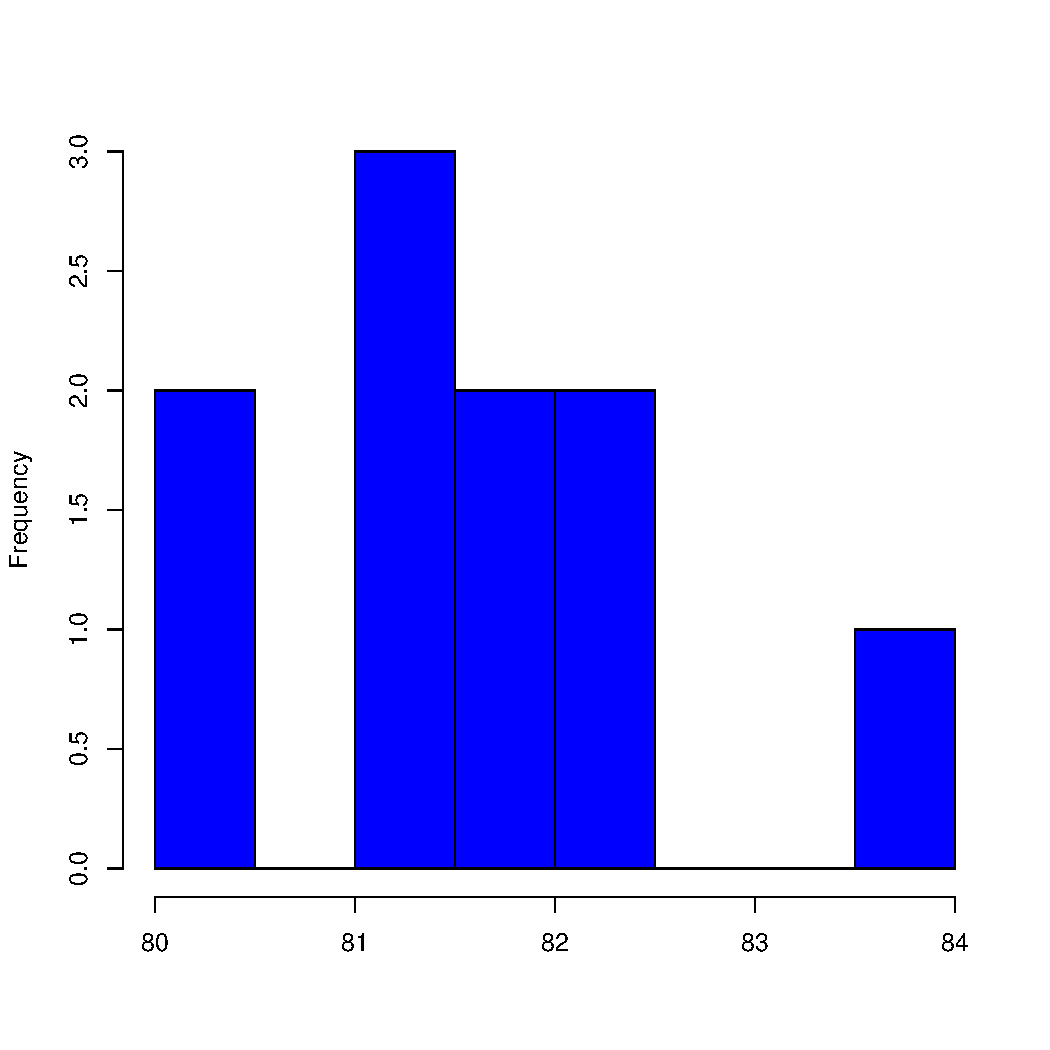
\includegraphics[width=\linewidth]{img/bluehist_afsa_cmfdr.pdf}
	\caption{Histograma dos ... do algoritmo AFSA (10 amostras)}
	\label{fig:hist_afsa_cmfdr}
\end{figure}

\begin{figure}[h]
	\centering
	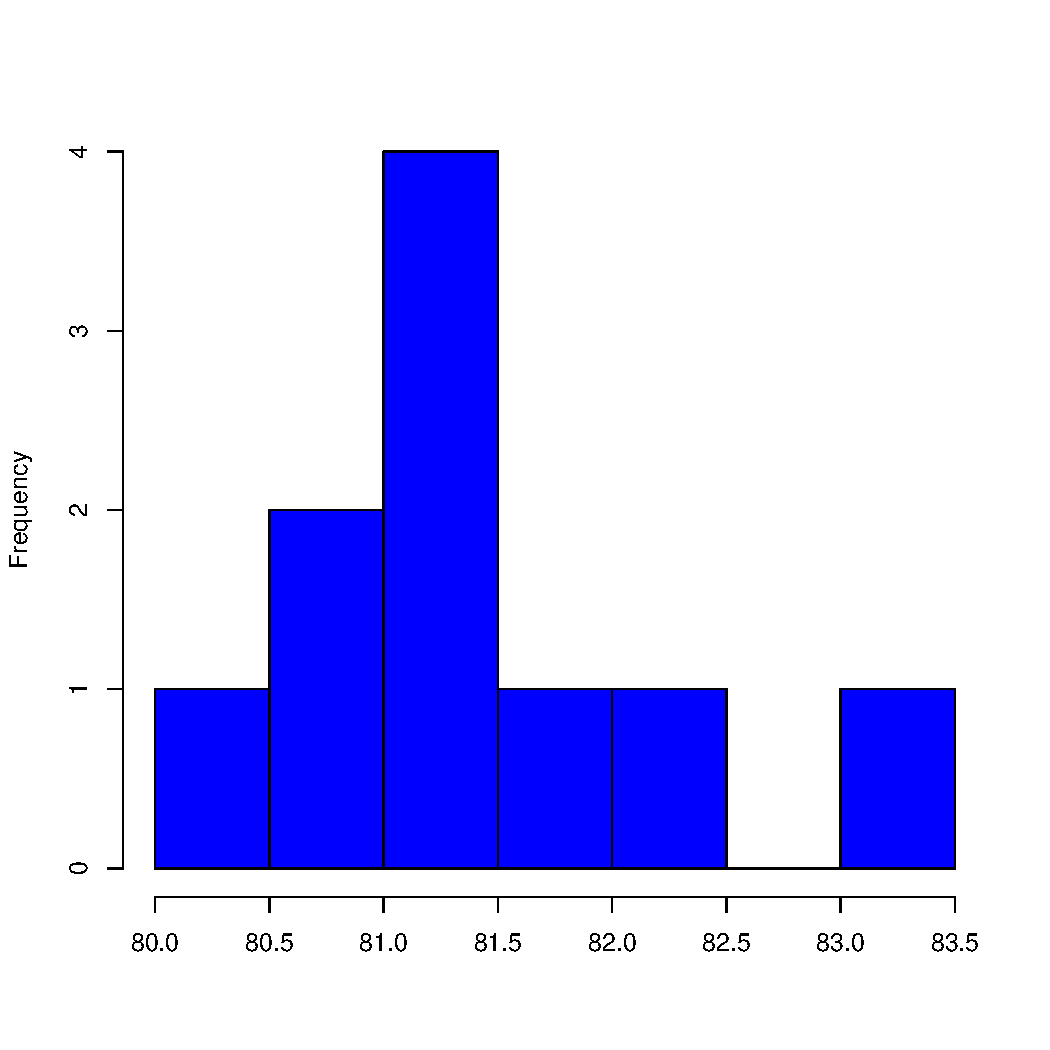
\includegraphics[width=\linewidth]{img/bluehist_cmfdr.pdf}
	\caption{\textcolor{red}{Escrever uma descrição}.}
	\label{fig:hist_cmfdr}
\end{figure}

\begin{figure}[h]
	\centering
	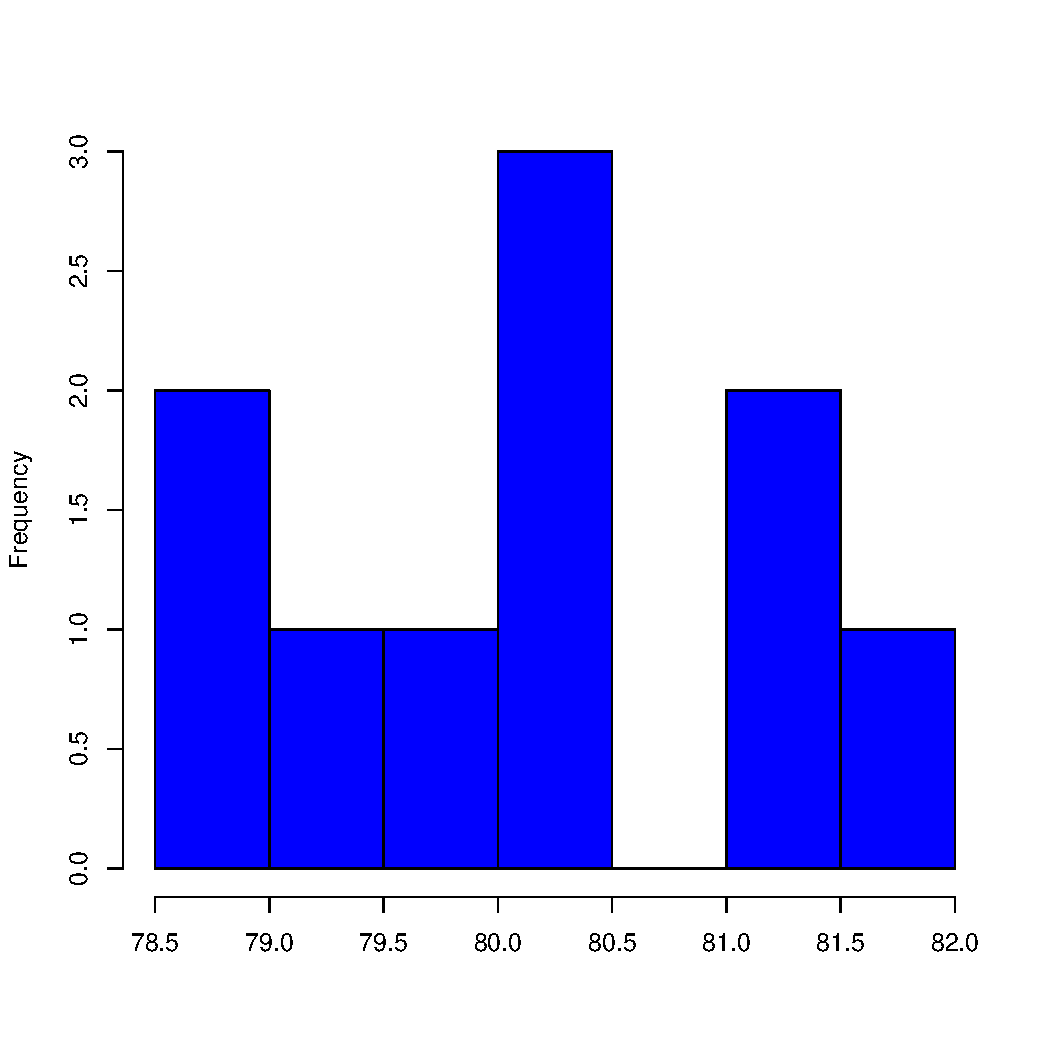
\includegraphics[width=\linewidth]{img/bluehist_afsa_mfdr.pdf}
	\caption{\textcolor{red}{Escrever uma descrição}.}
	\label{fig:hist_afsa_mfdr}
\end{figure}

\begin{figure}[h]
	\centering
	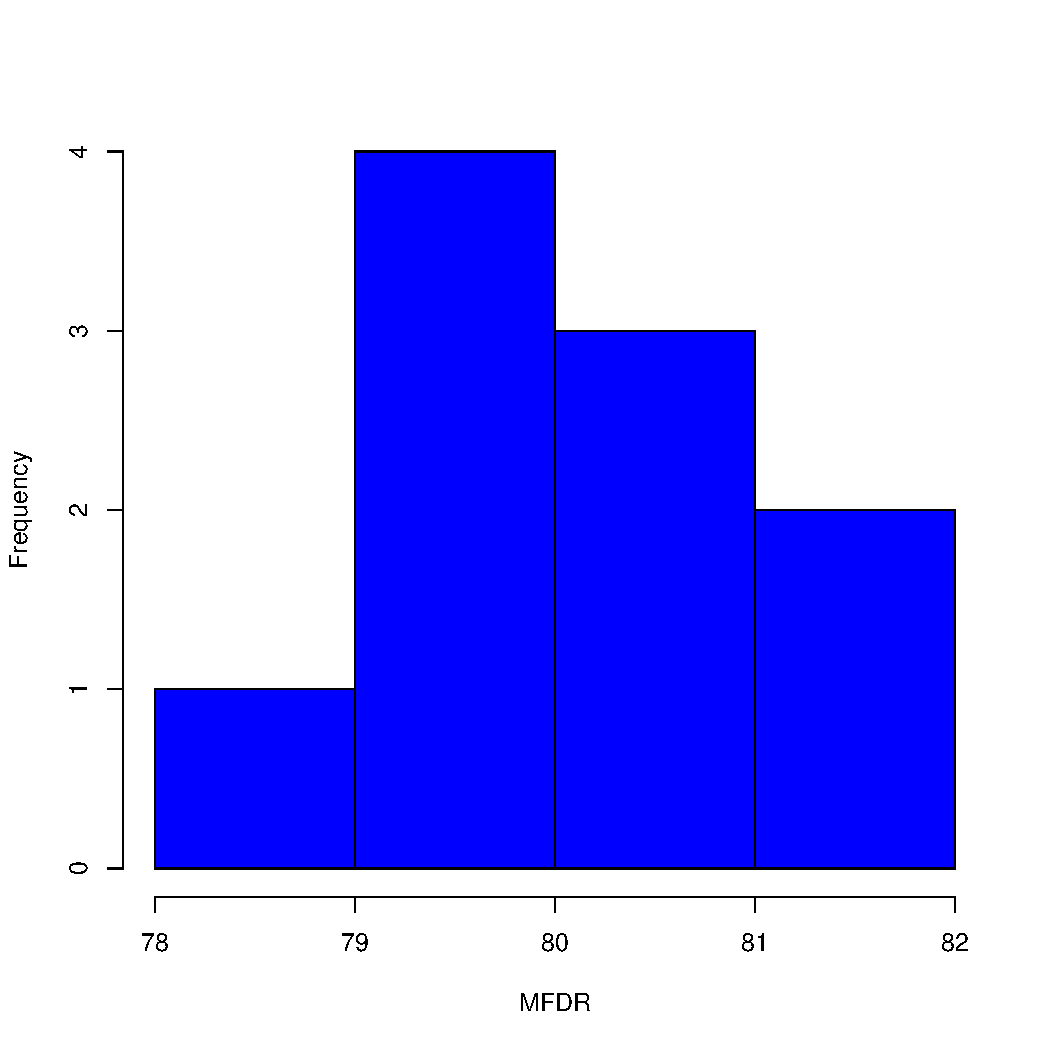
\includegraphics[width=\linewidth]{img/bluehist_mfdr.pdf}
	\caption{\textcolor{red}{Escrever uma descrição}.}
	\label{fig:hist_mfdr}
\end{figure}

\begin{figure}[h]
	\centering
	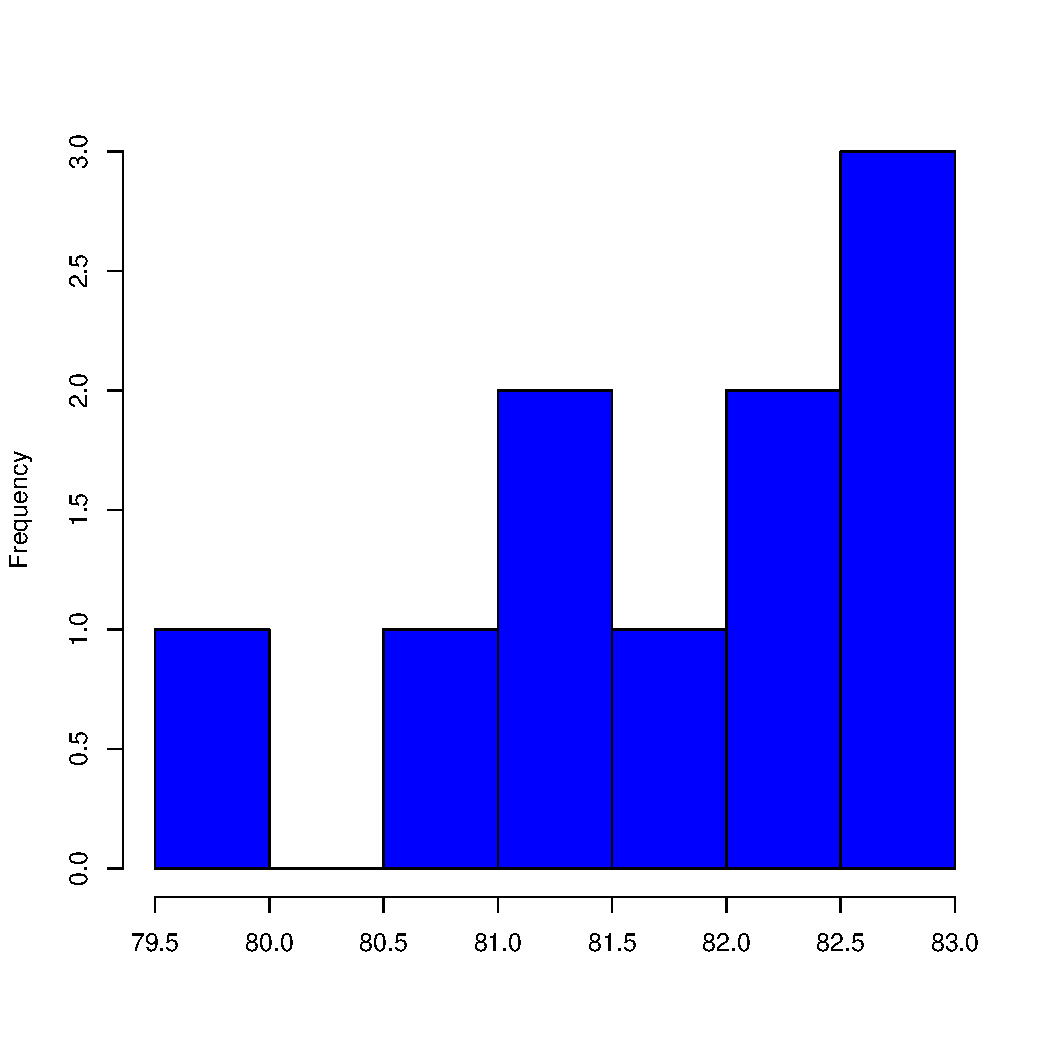
\includegraphics[width=\linewidth]{img/bluehist_afsa_mfd.pdf}
	\caption{\textcolor{red}{Escrever uma descrição}.}
	\label{fig:hist_afsa_mfd}
\end{figure}

\begin{figure}[h]
	\centering
	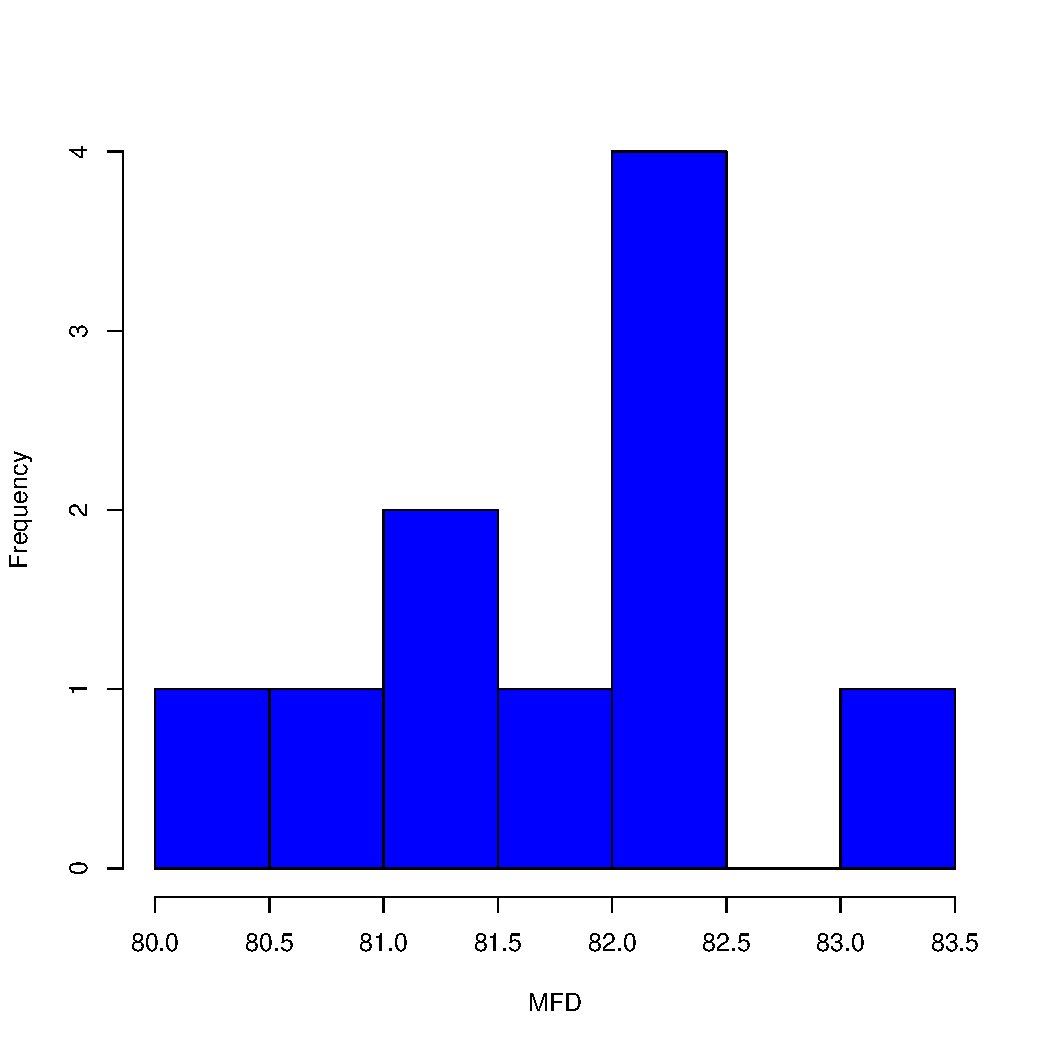
\includegraphics[width=\linewidth]{img/bluehist_mfd.pdf}
	\caption{\textcolor{red}{Escrever uma descrição}.}
	\label{fig:hist_mfd}
\end{figure}

A julgar pelos histogramas apresentados, não temos motivo para acreditar que tais amostras sejam provenientes de distribuições normais.
Para juntar mais evidências, continuaremos a análise com mais recursos.

Outra ferramenta visual útil é o \textcolor{red}{plot de probabilidade normal} ou \textit{normplots}, que permite verificar o quão bem os dados podem ser ajustados por uma distribuição normal.
Quando os dados são plotados dessa forma, uma linha reta indica uma distribuição normal ideal, sendo essa linha plotada para ser usada como referência.
Num cenário real, devido à presença de ruídos, não se espera que os dados se adequem perfeitamente à reta, porém se espera que, se os dados forem provenientes de uma distribuição normal, estes sejam bem aproximados pela reta de referência e estejam próximos a ela.
As Figuras \ref{} a \ref{} mostram os normplots de cada distribuição.

\begin{figure}[h]
	\centering
	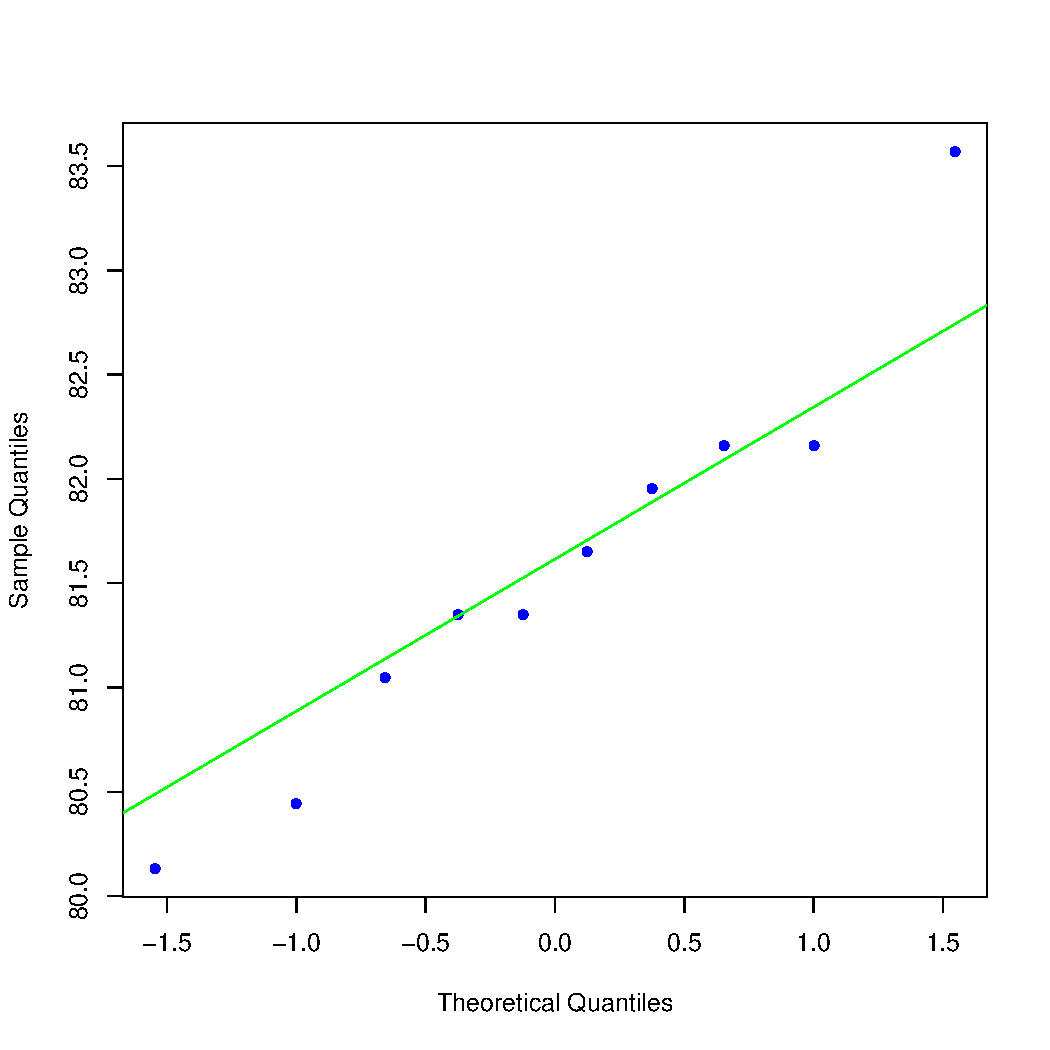
\includegraphics[width=\linewidth]{img/bluenorm_afsa_cmfdr.pdf}
	\caption{Normplot dos ... do algoritmo AFSA (10 amostras)}
	\label{fig:hist_afsa_cmfdr}
\end{figure}

\begin{figure}[h]
	\centering
	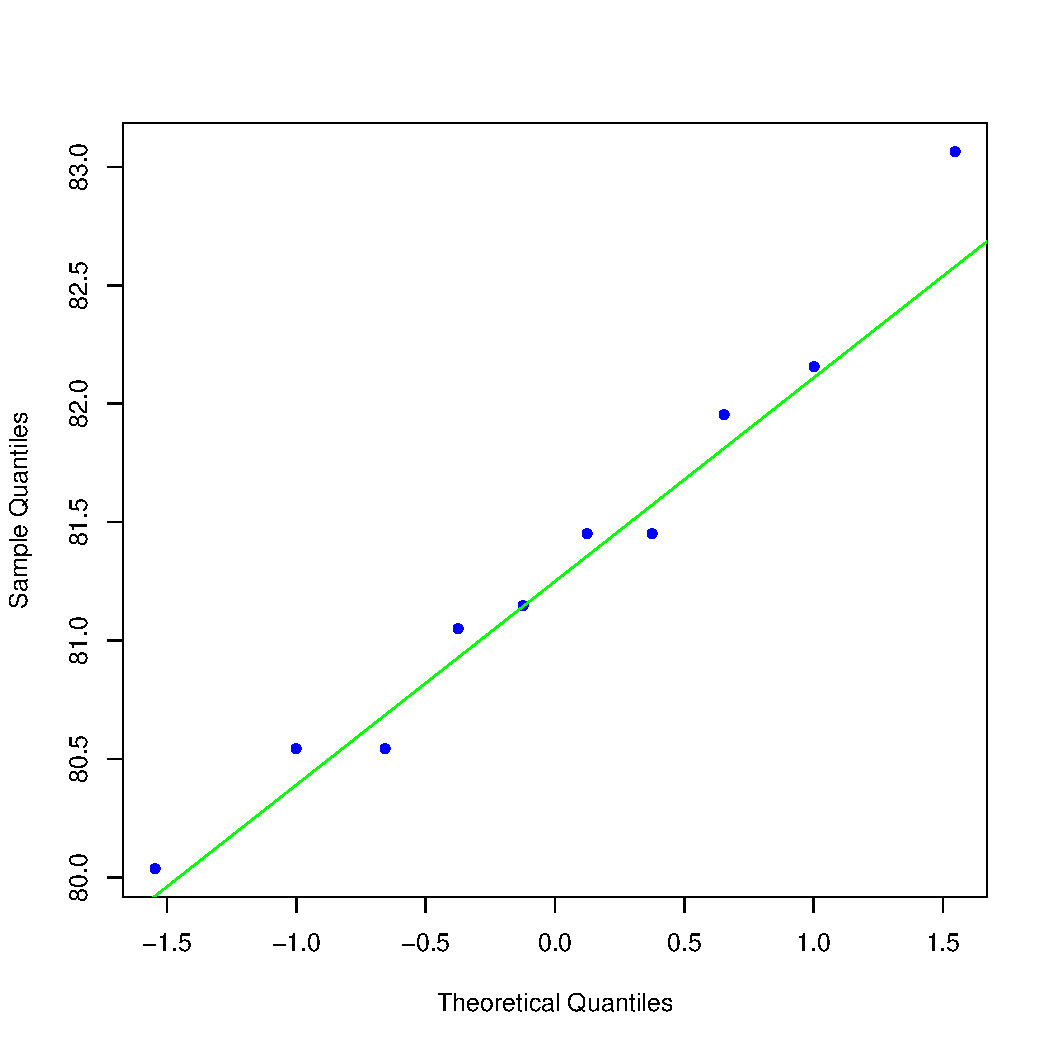
\includegraphics[width=\linewidth]{img/bluenorm_cmfdr.pdf}
	\caption{\textcolor{red}{Escrever uma descrição}.}
	\label{fig:hist_cmfdr}
\end{figure}

\begin{figure}[h]
	\centering
	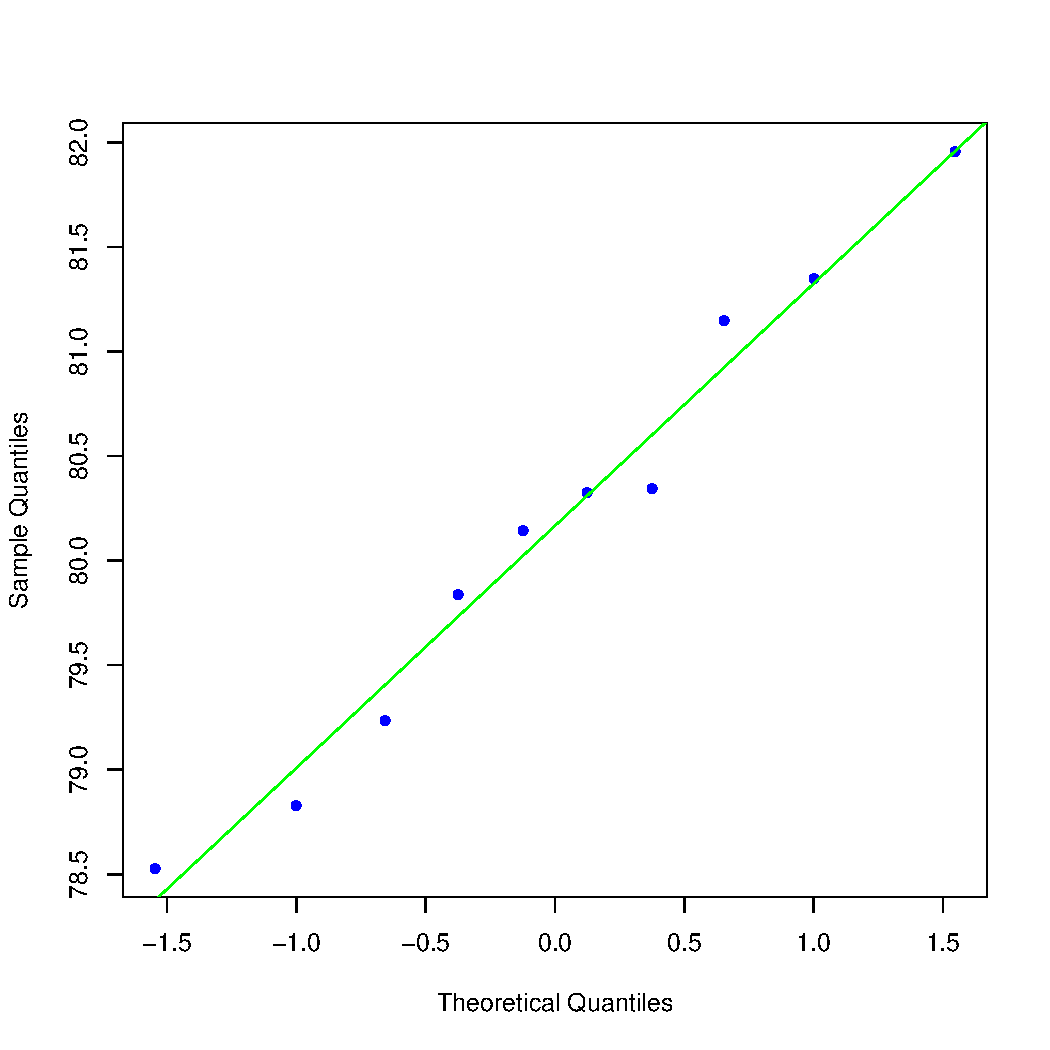
\includegraphics[width=\linewidth]{img/bluenorm_afsa_mfdr.pdf}
	\caption{\textcolor{red}{Escrever uma descrição}.}
	\label{fig:hist_afsa_mfdr}
\end{figure}

\begin{figure}[h]
	\centering
	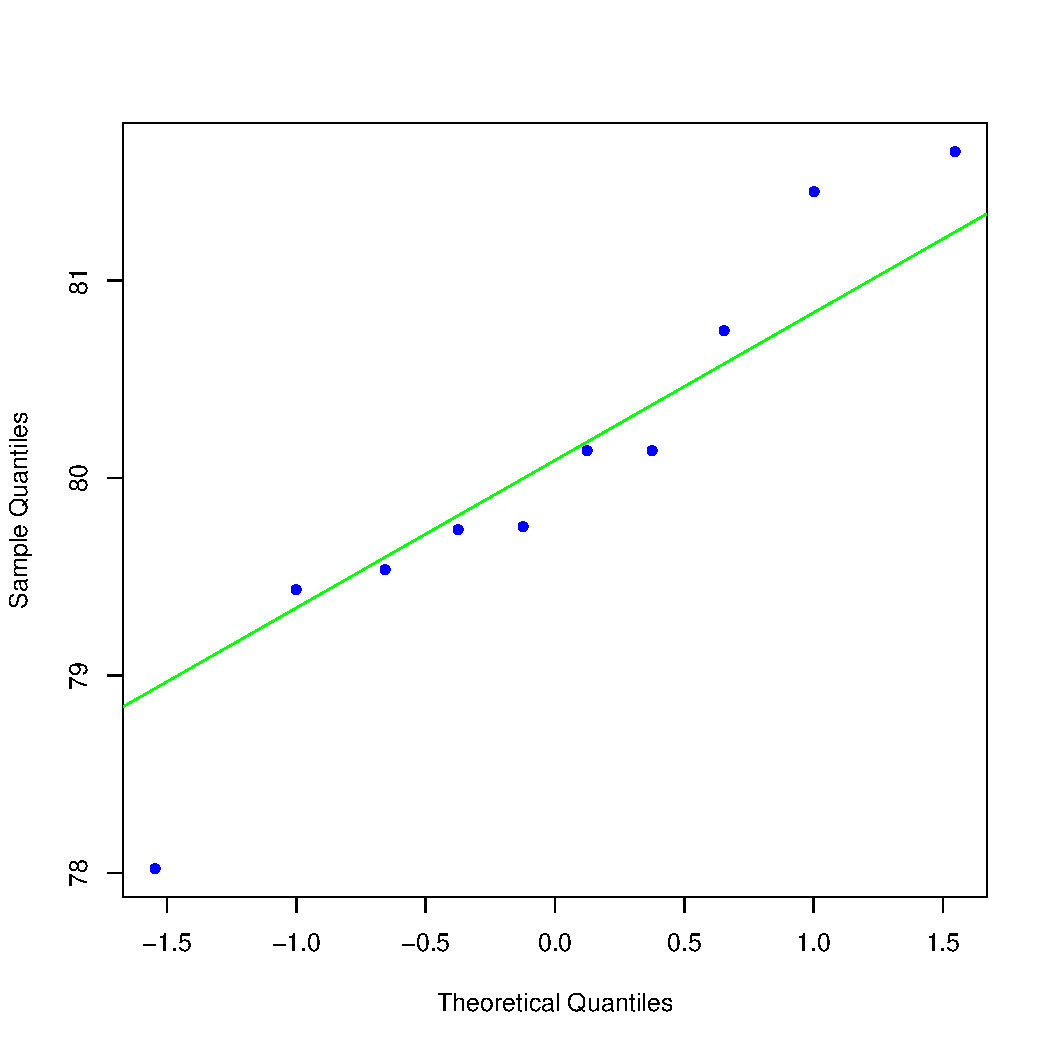
\includegraphics[width=\linewidth]{img/bluenorm_mfdr.pdf}
	\caption{\textcolor{red}{Escrever uma descrição}.}
	\label{fig:hist_mfdr}
\end{figure}

\begin{figure}[h]
	\centering
	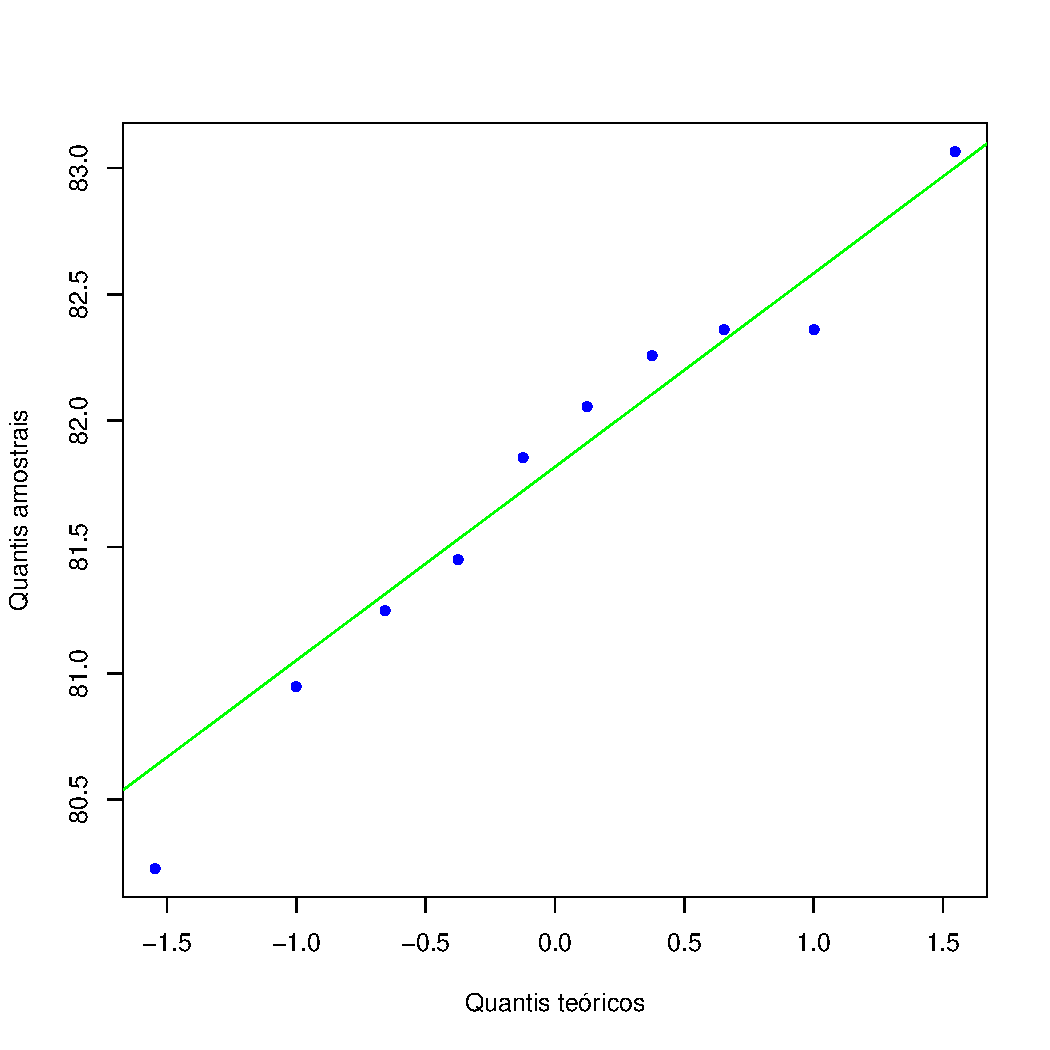
\includegraphics[width=\linewidth]{img/bluenorm_mfd.pdf}
	\caption{\textcolor{red}{Escrever uma descrição}.}
	\label{fig:hist_mfd}
\end{figure}


\begin{figure}[h]
	\centering
	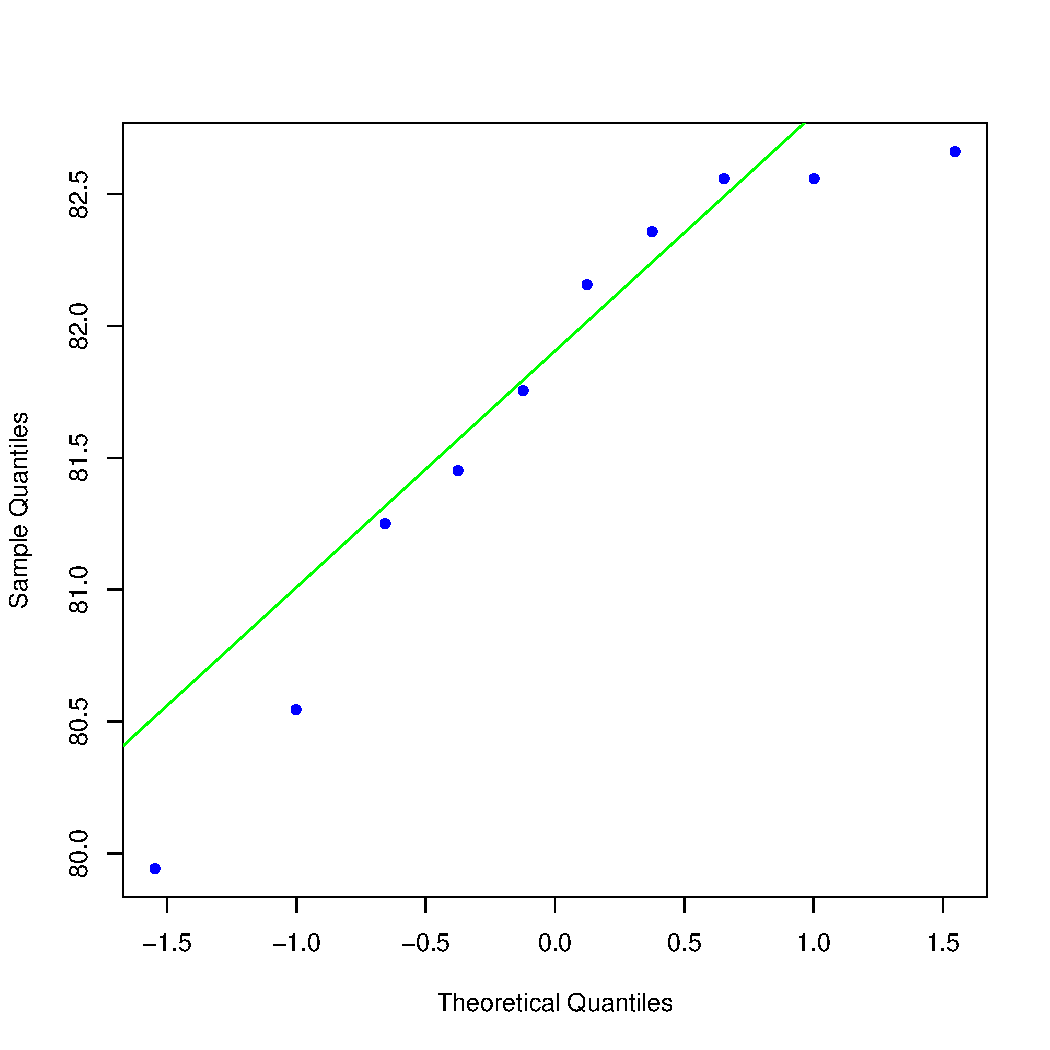
\includegraphics[width=\linewidth]{img/bluenorm_afsa_mfd.pdf}
	\caption{\textcolor{red}{Escrever uma descrição}.}
	\label{fig:hist_afas_mfd}
\end{figure}


\textcolor{red}{ISSUE: Os pontos não aparecem quando o latex importa o pdf Oo [Lucas: os pontos aparecem pra mim; além disso, minha impressão é que, se tivéssemos mais dados, os pontos se aproximariam da reta. Será que podemos afirmar que não é normal?]}

\textcolor{red}{[ROGÉRIO] Pra mim tb aparece}

Podemos observar que os dados não se aproximam tão bem de uma linha reta.

Por último ainda recorremos aos plot de caixa para verificar em particular a simetria dos dados. ...

Para confirmar nossa intuição de que as amostras não são normalmente distribuídas, recorremos a testes de hipótese utilizados para verificação de normalidade.
Os testes usados foram o de Shapiro-Wilk \cite{shapiro1965analysis} e ...	

\textcolor{red}{As amostras pequenas se mostraram um fator limitante da análise...}

\begin{table}[h]
	\centering
	\caption{Estatística descritiva}
	\label{tab:est_descr}
	\begin{tabular}{c|ccc}
		Método    & Média  & Mediana & Desv. Padrão  \\
		\hline
		AFSA cMFDR & 81.58186 	& 81.50202 	& 0.9741085 \\
		cMFDR & 81.3405 	& 81.3004 	& 0.8899744 \\
		AFSA MFDR & 80.16942 	& 80.23216 	& 1.109113 \\
		MFDR & 80.06198 	& 79.94699 	& 1.052274 \\
		AFSA MFD & 81.72414 	& 81.95565 	& 0.9268894 \\
		MFD & 81.78289 	& 81.95565 	& 0.824661 \\
		\hline
	\end{tabular}
\end{table}

\textcolor{red}{FALAR SOBRE OS RESULTADOS
Quais aparentam ser normais (média aprox. igual à mediana)
}


A Figura~\ref{fig:boxplot} apresenta uma.....

\begin{figure}[h]
	\centering
	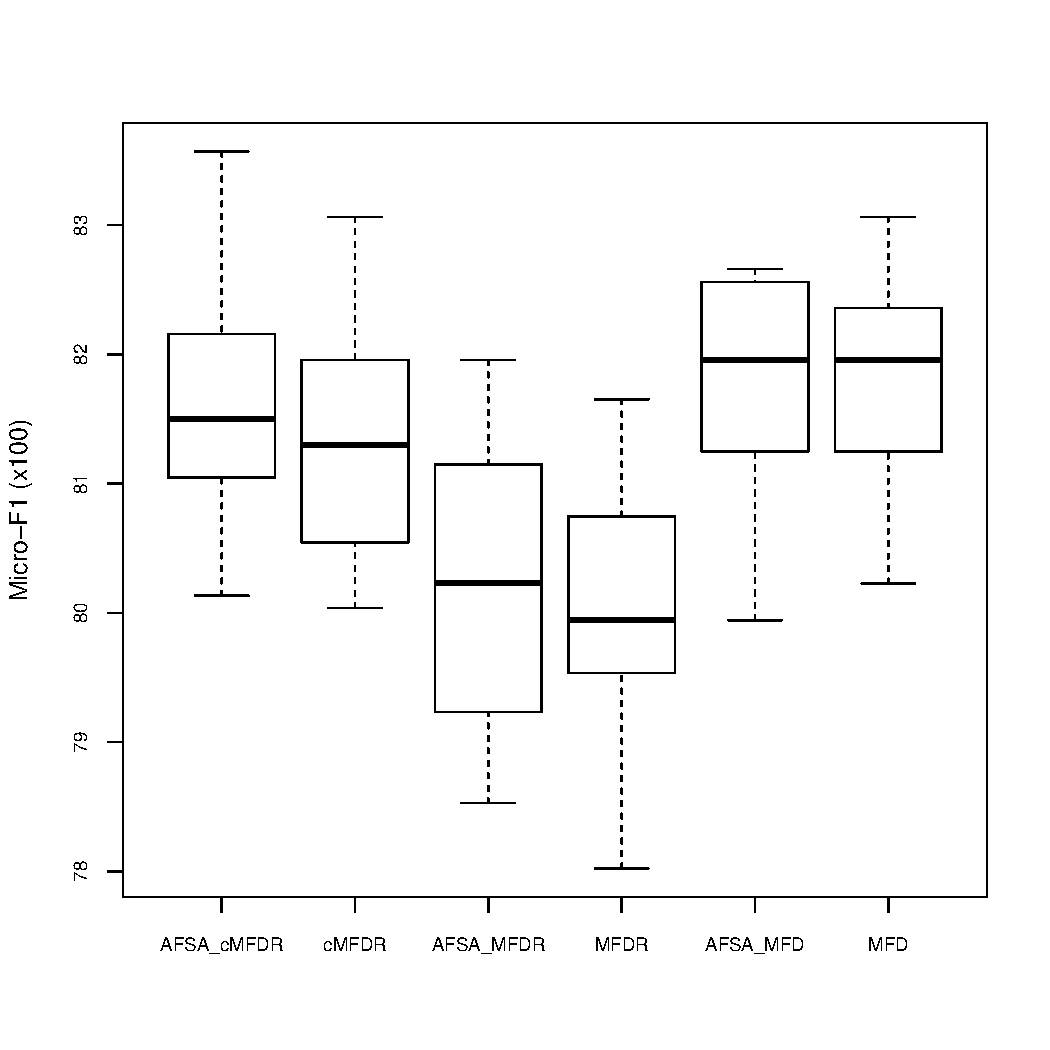
\includegraphics[width=\linewidth]{img/blueboxplot.pdf}
	\caption{\textcolor{red}{Escrever uma descrição}.}
	\label{fig:boxplot}
\end{figure}



\textcolor{red}{FAZER UMA CONCLUSÃO DA SEÇÃO
Falar das impressões sobre a normalidade dos dados com bases nos histogramas, boxplot e medidas estatísticas.......}

\subsection{Testes de aderência}

Uma maneira mais formal de verificar se as amostras seguem uma distribuição normal é com o uso de testes de aderência. Nesta pesquisa, foram executados os testes Shapiro-Wilk~\cite{shapiro1965analysis}, Anderson-Darling~\cite{anderson1954test} e Cramer-von Mises~\cite{durbin1972components}. Os resultados dos testes para cada amostra são apresentados na tabela~\ref{tab:aderencia}.

\begin{table}[h]
	\centering
	\caption{Resultados dos testes de aderência.}
	\label{tab:aderencia}
	\begin{tabular}{c|ccc}
		\hline
		& \multicolumn{3}{c}{\textit{p-value}}      \\
		\cline{2-4}
		& Shapiro-Wilk & Anderson-Darling  & Cramer-von Mises\\
		\hline
		AFSA CMFDR  	& 0.7513       & 0.6731           & 0.7485 \\
		cMFDR 				 & 0.9010       & 0.8626          & 0.8632 \\
		AFSA MFDR  		 & 0.8803       & 0.8929          & 0.8709 \\
		MFDR  				 & 0.6160       & 0.4717            & 0.4513 \\
		AFSA MFD   		  & 0.1950       &  0.2553          & 0.3081 \\
		MFD   				  & 0.8890       &  0.7704          & 0.7267 \\
		\hline
	\end{tabular}
\end{table}

Consideramos que uma amostra não segue uma distribuição normal caso o \textit{p-value} seja menor que 0.05. Deste modo, o resultado dos três testes apontam que, para todas as amostras, não existem evidências suficientes para rejeitar a hipótese nula de que a amostra segue uma distribuição normal, reforçando a impressão obtida da análise dos valores das médias e medianas das amostras~\ref{sec:estat_descr}. Porém é importante salientar que a eficiências de testes de aderência pode ser prejudicada quando as amostras são pequenas.Adicionalmente, a análise dos histogramas e dos boxplots (da maioria das amostras) dão indícios de que as amostras não seguem uma distribuição normal. Por estas razões, concluímos que, com os dados disponíveis, não temos segurança em afirmar que as amostras seguem uma distribuição normal. Diante disto, utilizamos teste de hipótese não-paramétrico para verificar a existência de diferenças significativas entre as amostras.


\subsection{Resultados}

Diante 

\section{Conclusão}
\label{sec:conclusao}

\textcolor{red}{Escrever conclusão}



\bibliographystyle{IEEEtran}
% argument is your BibTeX string definitions and bibliography database(s)
% \bibliography{IEEEabrv,../bib/paper}
\bibliography{bb}

\end{document}
